\documentclass[
    iict, % Saisir le nom de l'institut rattaché
    il, % Saisir le nom de l'orientation
    % confidential, % Décommentez si le travail est confidentiel
]{heig-tb}

\usepackage[nooldvoltagedirection,european,americaninductors]{circuitikz}

\signature{mbernasconi.svg} % Remplacer par votre propre signature vectorielle.

\makenomenclature
\makenoidxglossaries
\makeindex

\addbibresource{bibliography.bib}

\input{nomenclature}
\newacronym{gcd}{GCD}{Plus grand diviseur commun}
\newacronym{lcm}{LCM}{Plus petit multiple commun}
\newacronym{ide}{IDE}{Integrated Development Environment}
\newglossaryentry{heig-vd}{
  name=HEIG-VD,
  description={Haute École d'Ingénierie et de Gestion du canton de Vaud}
}
\newglossaryentry{hes-so}{
  name=HES-SO,
  description={Haute École Supérieure de Suisse Occidentale}
}
\newglossaryentry{latex}{
  name=latex,
  description={Un langage et un système de composition de documents}
}
\newglossaryentry{maths}{
  name=mathematics,
  description={Les mathematiques sont ce que les mathématiciens fonts}
}

% DE MOI DEPUIS ICI

\newglossaryentry{npm}{
  name=npm,
  description={Gestionnaire de paquets de l'environnement JavaScript et Node.js}
}

% Auteur du document (étudiant-e) en projet de Bachelor
\author{Valentin Kaelin}

% Activer l'option pour l'accord du féminin dans le texte
\genre{male}

% Titre de votre travail de Bachelor
\title{BeeScreens - b/place}

% Le sous titre est optionnel
\subtitle{Travail de Bachelor}

% Nom du professeur responsable
\teacher {Prof. N. Fatemi (HEIG-VD)}

% Mettre à jour avec la date de rendu du travail
\date{\today}

% Numéro de TB
\thesis{7212}



\surroundwithmdframed{minted}

%% Début du document
\begin{document}
\selectlanguage{french}
\maketitle
\frontmatter
\clearemptydoublepage

%% Requis par les dispositions générales des travaux de Bachelor
\preamble
\authentification

%% Résumé / Résumé publiable / Version abrégée
\begin{abstract}
  % contexte
L'association Baleinev organise depuis près de 30 ans le festival de musique Baleinev Festival sur le campus de l'HEIG.
Depuis 2014, le festival propose un concept innovant appelé Pimp My Wall. L'idée consiste à utiliser les fenêtres de l'école comme des écrans géants pour pouvoir notamment dessiner en temps réel depuis un smartphone.

Le concept a été repris de zéro en 2018 et a donné naissance à BeeScreens, la nouvelle version open source aux technologies modernes. Les ambitions ont été revues à la hausse avec l'idée de proposer de nombreuses applications interactives diffusées en continu sur Internet.
C'est dans ce contexte-ci qu'est né le projet de ce travail de Bachelor qui cherche à créer une
nouvelle application interactive à projeter entre autres sur un sous-ensemble des écrans du festival.

\asterism

% problématique
Le concept de BeePlace se base sur la conclusion que Pimp My Wall est une application trop permissive. Les utilisateurs peuvent dessiner de manière entièrement libre sur la toile virtuelle et cela engendre des comportements inappropriés.

% objectifs du travail
En recréant l'expérience proposée par le r/place de Reddit, l'objectif est de proposer une application web dans laquelle les utilisateurs peuvent créer des \oe{}uvres d'art collaboratives. Chaque utilisateur peut dessiner un pixel à la fois sur la toile et doit attendre un certain temps avant de pouvoir dessiner à nouveau. Cela permet de forcer la collaboration et de limiter les débordements.

Un des points principaux de ce travail en plus de la réalisation de l'application est d'assurer la montée en charge. L'application doit rester fluide dans le cas où de nombreuses personnes présentes au festival la rejoignent. Il est donc nécessaire de mettre en place des tests de montée en charge afin de pouvoir déterminer les limites de l'application et d'optimiser le code afin d'avoir des résultats satisfaisants.

% perspectives
Pour finir, le code de l'application a été pensé pour pouvoir être modifié, amélioré et étendu facilement pour s'adapter aux besoins futurs. Il ne s'agit pas d'un produit fini mais d'une base de travail pour les années à venir.

\end{abstract}

%% Sommaire et tables
\clearemptydoublepage
{
  \tableofcontents
  \let\cleardoublepage\clearpage
  \listoffigures
  \let\cleardoublepage\clearpage
  \listoftables
  \let\cleardoublepage\clearpage
  \listoflistings
}

\printnomenclature
\clearemptydoublepage
\pagenumbering{arabic}

%% Contenu
\mainmatter
\chapter{Introduction}
\section{Contexte}
L'association Baleinev organise, depuis plus de 25 ans, le festival de musique “Baleinev Festival” sur le campus de la HEIG-VD et aime se démarquer par son originalité.

En 2014, le festival proposait pour la première fois “Pimp My Wall”, un concept qui consiste à utiliser des fenêtres orientées sur la cour comme écrans géants, affichant du contenu interactif, des animations visuelles et la possibilité de dessiner à distance.

\begin{figure}[H]
  \centering
  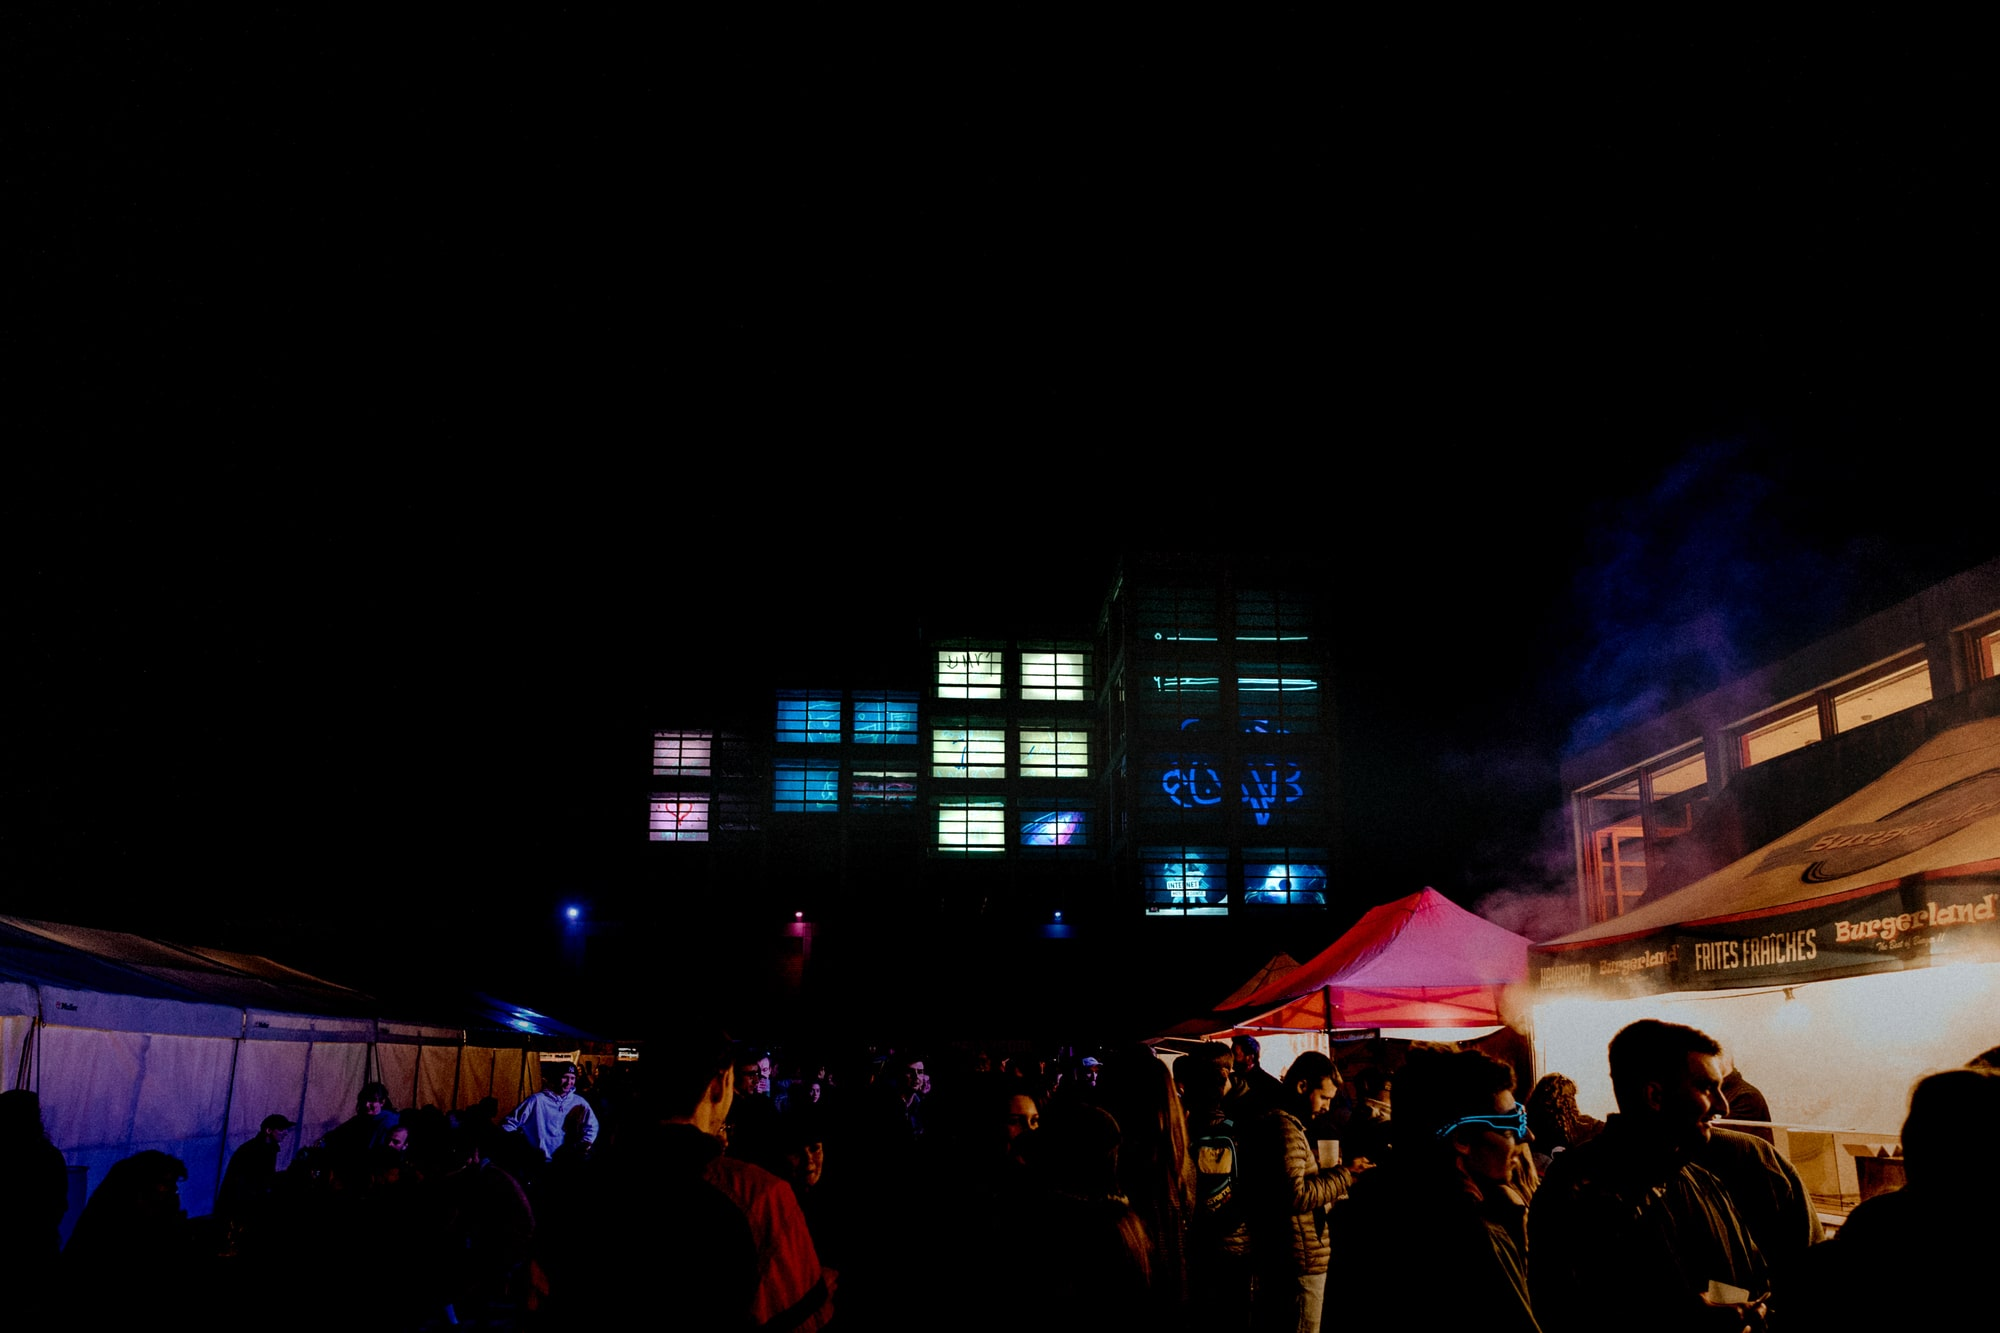
\includegraphics[width=0.8\textwidth]{assets/figures/pmw-ak.jpg}
  \begin{center}
    \textit{Photo réalisée par Antoine Kaelin}
  \end{center}
  \caption{Écrans de Pimp My Wall lors du Baleinev Festival 2023}
  \label{fig:pmw-baleinev-2023}
\end{figure}

En 2018, le concept a été repris à partir de zéro et a donné naissance à \gls{beescreens}, la nouvelle version open source aux technologies modernes. L'ambition est de concevoir un système permettant le développement d'applications interactives diffusées en continu sur Internet (applications, jeux, multi-joueurs, multi-écrans, tout est imaginable). L'idée n'est plus de se limiter uniquement au Baleinev festival mais de pouvoir utiliser les applications développées dans d'autres situations.

C'est dans ce contexte qu'est né le projet de ce travail de Bachelor avec la volonté de créer une nouvelle application interactive à projeter entre autres sur un sous-ensemble des écrans du festival.

\section{Présentation r/place}
\gls{reddit} (\href{https://www.reddit.com}{reddit.com}), sûrement le forum en ligne le plus connu au monde, a l'habitude de faire des expériences pour le premier avril. En 2017, \gls{reddit} présente pour la première fois leur concept r/place.

r/place~\cite{rplace} offre une toile géante virtuelle permettant à tout le monde de placer un pixel d'une couleur choisie parmi une liste prédéfinie. Chaque personne doit attendre un certain temps (5 minutes) avant de reposer un nouveau pixel. Cela oblige une collaboration des utilisateurs afin de réaliser des dessins de qualité, ce qui implique qu'aucun individu ou groupe ne peut nuire trop fortement à l'ensemble de l'\oe{}uvre.

En 2022, une nouvelle version du r/place est mise en place et plus de 6 millions de personnes participent à cette édition. La toile est agrandie pour atteindre des dimensions de 2000x2000 pixels et celle-ci se trouve remplie de créations en tout genre réalisées par diverses communautés (voir figure \ref{fig:rplace2022}) pendant plusieurs jours.

\begin{figure}[H]
  \centering
  
\includegraphics[width=0.8\textwidth]{./assets/figures/rplace.png}
  \caption{Résultat du r/place de 2022}
  \label{fig:rplace2022}
\end{figure}

Les codes sources de ces deux événements ne sont malheureusement pas disponibles. Cependant, les ingénieurs du r/place ont publié des articles présentant leur architecture et leur implémentation. Ces articles sont disponibles sur le site de \gls{reddit}~\cite{rplace2017, rplace2022}. Ces articles seront utilisés comme référence pour ce travail de Bachelor mais l'architecture ainsi que l'implémentation seront complètement différentes. En effet, le but est de créer seul une version open source de r/place. L'envergure du projet ainsi que la taille du public visé sont évidemment bien moindres que ceux du r/place original.

\section{Cahier des charges}
\label{sec:cdc}

\subsection{Objectifs}

Le but principal de ce travail de Bachelor consiste à recréer une version open source du fameux r/place de \gls{reddit}. Cette variante sera nommée \gls{beeplace} afin de s'aligner avec le nom de l'écosystème \gls{beescreens}.
Cette application, comme le r/place original, a comme objectif de permettre aux utilisateurs de poser des pixels sur une toile virtuelle partagée entre tous. Chaque utilisateur pourra poser un ou plusieurs pixels d'une couleur choisie parmi une liste prédéfinie. Afin de maximiser la collaboration entre les utilisateurs, ceux-ci devront attendre un certain délai entre chaque pose de pixel. Ce délai a également pour visée de minimiser les dégâts causés par des utilisateurs malveillants qui pourraient vouloir détruire les \oe{}uvres des autres utilisateurs ou dessiner des images inappropriées.

En plus de l'application en elle-même, des critères non-fonctionnels sont à prendre en compte. Tout d'abord, il est nécessaire d'assurer sa montée en charge afin qu'elle puisse supporter des possibles hausses de fréquentation, notamment le soir du festival. Ce critère sera vérifié grâce à des tests prévus à cet effet. De plus, il est important d'assurer l'intégration continue de l'application au sein de l'écosystème \gls{beescreens}. En effet, \gls{beeplace} fera partie intégrante de l'écosystème existant et devra donc être correctement intégrée afin de pouvoir être facilement utilisée dans le futur. Pour finir, l'application doit être agréable d'utilisation sur téléphone car les utilisateurs du festival utiliseront principalement ce moyen d'interaction.

\subsection{Fonctionnalités}

Afin d'avoir une idée plus précise des tâches à réaliser, les diverses fonctionnalités de l'application ont été listées. Celles-ci sont catégorisées selon leur importance. Les fonctionnalités \textbf{required} sont nécessaires au bon fonctionnement de l'application. Les \textbf{essential} aident beaucoup à la qualité du projet final et pour finir les \textbf{nice-to-have} améliorent surtout l'expérience utilisateur des usagers ainsi que des administrateurs qui ont la tâche de supprimer les éventuels débordements.

\subsubsection{Fonctionnalités \guillemotleft required\guillemotright}

\begin{itemize}
  \item L'utilisateur arrive sur une page affichant la toile virtuelle au complet.
  \item La toile s'actualise avec les modifications réalisées par les autres utilisateurs.
  \item L'utilisateur peut zoomer ou dézoomer sur la toile afin de voir les moindres détails.
  \item L'utilisateur voit facilement le nombre de pixels qu'il a actuellement la possibilité de placer sur la toile.
  \item L'utilisateur peut sélectionner un pixel, choisir une couleur parmi plusieurs proposées et le colorier.
  \item Les dimensions de la toile doivent être configurables par un administrateur.
  \item L'utilisateur dispose d'un moyen de recharger ses pixels à placer une fois ceux-ci écoulés. Il peut par exemple recevoir un nombre de pixels définis après un temps d'attente également choisi.
\end{itemize}

\subsubsection{Fonctionnalités \guillemotleft essential\guillemotright}

\begin{itemize}
  \item Il doit être possible, pour un administrateur, de passer la toile dans un mode “lecture uniquement” pour tous les utilisateurs.
  \item Créer des tests de montée en charge de l'application afin d'assurer un bon fonctionnement lors des festivals notamment.
  \item Afin d'éviter que les utilisateurs puissent recharger la page pour recevoir à nouveau des pixels, trouver un moyen de les identifier.
  \item Les coordonnées du pixel sélectionné par l'utilisateur lui sont affichées ainsi que son niveau de zoom.
  \item Créer des tests unitaires ainsi que des tests d'intégration pour s'assurer de la qualité de l'application.
  \item Un administrateur peut choisir une zone à censurer (recouvrir/suppression de pixels d'une couleur) à partir d'un call API en cas de comportement non désiré.
\end{itemize}

\subsubsection{Fonctionnalités \guillemotleft nice-to-have\guillemotright}

\begin{itemize}
  \item Ajouter une interface utilisateur permettant aux administrateurs de censurer plus facilement une zone de la toile via le dashboard.
  \item Une fois ses pixels épuisés, l'utilisateur peut les recharger via un moyen physique.
  \item Faire en sorte que les couleurs disponibles aux utilisateurs soient facilement customisables par l'administrateur (ex: via le dashboard).
  \item Les administrateurs peuvent interdire la pose de pixels à des utilisateurs ou des régions spécifiques.
  \item Les administrateurs peuvent changer la taille de la toile dynamiquement (ex : via le dashboard).
  \item Afficher à chaque utilisateur le nombre de festivaliers actuellement connectés sur la toile.
  \item Développer un mode “affichage”, permettant d'afficher régulièrement un code QR pour rejoindre la toile virtuelle. En plus de ce code QR, ajouter des éléments sollicitant l'interaction de l'utilisateur à la manière d'un économiseur d'écran (ex: des pixels qui s'animent de façon indépendante). Ce mode s'enlèverait automatiquement dès qu'un utilisateur est actif sur l'application.
  \item Ajouter la possibilité de sauvegarder le dessin.
  \item Intégrer la notion de CRDTs (Conflict-free Replicated Data Type), une structure de données permettant d'éviter les conflits notamment dans les systèmes distribués collaboratifs multi utilisateurs.
\end{itemize}

\subsection{Calendrier}

Le projet est séparé en différentes milestones, les dates de celles-ci sont adaptées en fonction des événements clés du semestre, comme les délais de rendu ainsi que le festival Baleinev 2023 en lui-même.

\subsubsection{Milestone 1 - semaine du 20 au 26 mars}

\begin{enumerate}
  \item Rédaction du cahier des charges
  \item Rédaction de la partie du rapport concernant l'intégration dans l'environnement \gls{beescreens}
\end{enumerate}

\subsubsection{Milestone 2 - semaine du 17 au 23 avril}

\begin{enumerate}
  \item Intégration à l'environnement \gls{beescreens} de l'application \gls{beeplace}
  \item Réalisation d'une première version de l'application afin d'être potentiellement utilisée lors du festival Baleinev de cette année
\end{enumerate}

\subsubsection{Milestone 3 - semaine du 22 au 28 mai}
\label{milestone3}

\begin{enumerate}
  \item Rédaction du rapport intermédiaire
  \item Utilisation d'outils de tests de montée en charge afin d'identifier les problèmes du code actuel
\end{enumerate}

\subsubsection{Milestone 4 - semaine du 12 au 18 juin}

\begin{enumerate}
  \item Optimisation de l'application afin d'améliorer sa scalabilité
  \item Potentiels tests avec les CRDTs (Conflict-free Replicated Data Type)
\end{enumerate}

\subsubsection{Milestone 5 - semaine du 24 au 30 juillet}

\begin{enumerate}
  \item Réalisation des derniers livrables: le résumé publiable ainsi que le poster
  \item Finalisation du rapport
  \item Implémentation de fonctionnalités “nice-to-have”
\end{enumerate}

Le travail se termine le jeudi 27 juillet avec la remise du rapport et des autres livrables indiqués ci-dessous. La défense du travail aura lieu dans les semaines qui suivent.

\subsection{Livrables}

Les livrables à réaliser pour ce travail de Bachelor sont les suivants:

\begin{itemize}
  \item L'application BeePlace;
  \item Un rapport intermédiaire;
  \item Un rapport final;
  \item Un résumé publiable;
  \item Un poster.
\end{itemize}



\chapter{Intégration à l'environmement BeeScreens}
\section{Environnement existant}

Le code de tous les projets existants réalisés par l'équipe BeeScreen se trouvent dans un unique répertoire GitLab \cite{beescreens}. En effet, le répertoire est organisé sous la forme d'un monorepo. Ce qui signifie, qu'au lieu d'avoir une répertoire par projet comme il était surtout courant auparavant, tous les projets sont regroupés. Cette pratique a émergé au début des années 2000, notamment grâce aux grands noms de la tech comme Google, Meta ou encore Airbnb. Cela facilite notamment la collaboration entre les développeurs en ayant directement accès au code complet.

Le répertoire est organisé grâce à une workspace pnpm \cite{pnpmworkspace} afin de gérer le fait qu'il s'agit d'un monorepo. Un fichier de configuration est créé à la racines du répertoire en spécifiant la liste et le chemins vers tous les projets contenus dans le répertoire. Cela permettant notamment d'installer les dépendances de tous les projets en une seule commande.

pnpm est une version améliorée du gestionnaire de paquets par défaut présent avec Node.js npm. Il permet notamment de gérer les dépendances de manière plus efficace en utilisant des liens symboliques afin de ne pas avoir à copier les dépendances dans le dossier \mintinline[breaklines]{bash}{node_modules} de chaque projet. Cela permet de gagner en temps de compilation et en espace disque. De plus, comme évoqué précédemment, pnpm permet une gestion des monorepos plus efficace grâce à la notion de workspace.

\subsection{Structure du répertoire}

\dirtree{%
  .1 /.
  .2 apps.
  .3 media-player.
  .3 pimp-my-wall.
  .2 deployement.
  .3 apps.
  .4 ....
  .3 cicd.
  .3 infra.
  .2 docs.
  .2 packages.
  .3 pimp-my-wall.
}

Le dossier \mintinline[breaklines]{bash}{apps} contient les applications déjà développées qui sont pour l'instant:

\begin{enumerate}
  \item Media Player : une application permettant de lire des images ainsi que des vidéos afin d'afficher entre autre les sponsors et diverses informations lors du festival sous forme de diaporama.
  \item Pimp My Wall : l'application majeure du projet permettant aux utilisateurs de collaborer en temps réel en dessinant sur la même toile virtuelle. Cette application pourra servir de point de repère lors du développement de l'application BeePlace comme ces deux applications ont des fonctionnalités similaires (ex: temps réel, canvas partagé entre les utilisateurs, etc.).
\end{enumerate}

Le dossier \mintinline[breaklines]{bash}{deployement} contient les fichiers nécessaires au déploiement des diverses applications à l'aide de Docker ainsi que de Docker Compose. Chaque application possède son propre dossier à l'intérieur du dossier \mintinline[breaklines]{bash}{deployment/apps}. Les dossiers \mintinline[breaklines]{bash}{cicd} et \mintinline[breaklines]{bash}{infra} contiennent surtout des instructions sur la configuration des Raspberry Pis, utilisés afin de projeter les créations des utilisateurs de Pimp My Wall sur les murs du festival.

Le dossier \mintinline[breaklines]{bash}{docs} contient le code source de la documentation en ligne du projet \cite{beescreensdocs}. Celle-ci contient notamment divers tutoriels afin de créer de zéro des versions simplifiées des applications développées par l'équipe BeeScreens. De plus, divers guides ont également été créés afin de faciliter la prise en main des technologies utilisées dans le répertoire.

Pour finir, dossier \mintinline[breaklines]{bash}{packages} contient les différents paquets \Gls{npm} utilisés pour partager du code entre différentes applications (ex: entre la partie client et serveur d'une application).

% \subsection{CI/CD}

% TODO: CI/CD GitLab, déploiement

% \subsection{Tests}

% TODO: tests, husky

\subsection{Lien avec le projet BeePlace}
\label{sec:lien-avec-le-projet-beeplace}

BeePlace est une nouvelle application indépendante des applications existantes du projet BeeScreens. Cependant, comme expliqué précédemment, BeeScreens étant un monorepo, l'application BeePlace doit être ajoutée au même répertoire.

L'idée de BeePlace est arrivée suite aux conclusions réalisées à propos de l'application existante, Pimp My Wall. La problématique est la suivante: Pimp My Wall est une application trop permissive. Les utilisateurs peuvent dessiner de manière entièrement libre sur la toile virtuelle et cela donne suite à des comportements inappropriés. Le public cible, les festivaliers de Baleinev, est relativement jeune et l'ambiance festive de la soirée amène plus facilement à des dérives. Comme les créations des festivaliers sont affichés en temps réel sur les murs de l'école, il est nécessaire de modérer les créations des utilisateurs. Cette modération est fastidieuse, peu gratifiante et demande beaucoup de temps.

Afin de pallier à ce problème, l'idée de BeePlace est née. En imposant un délai entre la pose de pixels aux utilisateurs, ceux-ci seront moins enclins à réaliser des créations inadaptées car cela leur demanderait un effort plus conséquent. Dans le cas où des débordements auraient quand même lieu, la modération pourrait remettre à zéro une zone de la toile en quelques clics. Ce qui ferait perdre énormément de temps aux usagers problématiques et les dissuaderait de recommencer.

\section{Intégration}

Pour réaliser l'intégration de façon optimale, un guide \cite{addapptobeescreens} a été créé par les mainteneurs du projet BeeScreens expliquant les étapes à suivre afin d'ajouter une nouvelle application au répertoire.

\subsection{Création d'une nouvelle application}

La première étape consiste à créer le dossier de l'application dans le dossier \mintinline[breaklines]{bash}{apps} décrit précédemment. Dans celui-ci, deux dossiers sont également créés: \mintinline[breaklines]{bash}{frontend} et \mintinline[breaklines]{bash}{backend}. Le premier contient le code source de l'application côté client tandis que le second contient le code source de l'application côté serveur. D'éventuels autres dossiers seront peut être nécessaires en fonction des besoins de l'application. Ceux-ci seront créés après l'analyse préliminaire permettant de choisir les technologies utilisées.

L'arborescence est donc actuellement la suivante:

\dirtree{%
  .1 /.
  .2 apps.
  .3 beeplace.
  .4 backend.
  .4 frontend.
  .3 ....
  .2 ....
}

Par la suite, un fichier \mintinline[breaklines]{bash}{package.json} est nécessaire par dossier. Ces fichiers sont normalement utilisés dans les projets JavaScript et Node.js afin de préciser notamment les scripts, les dépendances et diverses métadonnées du projet. Dans ce cas-ci, ils sont utilisés peu importe les technologies qui seront choisies pour ce projet. En effet, cela permet d'unifier beaucoup d'aspects sur l'entièreté du code BeeScreens. Par exemple, il est possible de lancer les tests unitaires de toutes les applications grâce au fichier \mintinline[breaklines]{bash}{package.json} créé à la racine du répertoire. Si la future application n'est pas développée en JavaScript, les scripts du \mintinline[breaklines]{bash}{package.json} lancerons les commandes nécessaires dans le langage souhaité afin d'abstraire le plus possible les technologies utilisées.

La structure des fichiers \mintinline[breaklines]{bash}{package.json} est basée sur celle suggérée par les mainteneurs BeeScreens \cite{aboutpnpmbeescreens}. De nombreuses clés sont omises pour l'instant comme les technologies ne sont pas encore définies. La structure actuelle est la suivante:

\begin{listing}[h]
  \inputminted{json}{assets/figures/package.json}
  \caption{package.json initial du Backend l'application BeePlace}
\end{listing}

Celui du frontend suit la même structure. Un script de test a été ajouté afin de vérifier que l'intégration est réussie par la suite.

Un dossier ainsi qu'un fichier \mintinline[breaklines]{bash}{package.json} peuvent être créés dans le dossier \mintinline[breaklines]{bash}{packages} si du code doit être partagé entre les diverses parties de l'application. Ce besoin n'a pas encore été identifié donc aucun package n'a pour le moment été créé.

\subsection{Ajouter l'application au monorepo}

Afin de prévenir pnpm qu'une nouvelle application a été ajoutée à la workspace, il faut modifier le fichier \mintinline[breaklines]{bash}{pnpm-workspace.yaml} présent à la racine du répertoire en ajoutant les chemins vers les deux applications créées précédemment.


Grâce à cela, il est possible de lancer les tests précédemment créés en filtrant sur les applications souhaitées afin d'observer les résultats affichés dans le terminal.

\begin{minted}{bash}
  pnpm \
  --filter @beescreens/beeplace-backend \
  --filter @beescreens/beeplace-frontend \
  test

  # Résultat
  Scope: 2 of 11 workspace projects
  apps/beeplace/frontend test$ echo "This is a test from BeePlace Frontend!"
  │ This is a test from BeePlace Frontend!
  └─ Done in 9ms
  apps/beeplace/backend test$ echo "This is a test from BeePlace Backend!"
  │ This is a test from BeePlace Backend!
  └─ Done in 9ms
\end{minted}

Afin d'être sûr que l'IDE VSCode ait connaissance de la nouvelle application, il est également nécessaire d'ajouter les chemins dans le fichier de configuration \mintinline[breaklines]{bash}{.vscode/settings.json} présent à la racine du répertoire.

\subsection{CI/CD}

L'application doit être intégrées à deux pipelines: la locale gérée via Husky et la pipeline GitLab. Pour la première, il faut ajouter au fichier \mintinline[breaklines]{bash}{.husky/pre-push} le code suivant afin de lancer les tests avant chaque push:

\begin{minted}{bash}
## BeePlace
if
  did_files_change_in_directory "apps/beeplace/**/*"
then
  ## test
  pnpm --parallel \
  --filter @beescreens/beeplace-backend \
  --filter @beescreens/beeplace-frontend \
  test
fi
\end{minted}

Grâce à la fonction \mintinline[breaklines]{bash}{did_files_change_in_directory}, les tests ne seront lancés que si des fichiers ont été modifiés dans le dossier de l'application.

Pour la pipeline GitLab, il faut tout d'abord créer un nouveau fichier \mintinline[breaklines]{bash}{.gitlab/ci_cd/beeplace.yml}. Celui-ci contient les différentes étapes de la pipeline. Pour l'instant, il n'y a que la première étape qui est nécessaire: le lancement des "tests".

\begin{minted}{yaml}
## Backend

# test
beeplace::app::backend::test:
  needs:
  - setup env
  extends: .test
  variables:
  PROJECT_PATH: "apps/beeplace/backend"
  PROJECT_NAME: "@beescreens/beeplace-backend"
  script:
  - echo "Testing $PROJECT_NAME..."

## Frontend

# test
beeplace::app::frontend::test:
  needs:
  - setup env
  extends: .test
  variables:
  PROJECT_PATH: "apps/beeplace/frontend"
  PROJECT_NAME: "@beescreens/beeplace-frontend"
  script:
  - echo "Testing $PROJECT_NAME..."
\end{minted}

Ce fichier doit être inclus dans le fichier \mintinline[breaklines]{bash}{.gitlab/ci_cd/main.yml} afin d'être ajouté à la pipeline globale.

L'application est maintenant prête à être développée. Le code peut être push afin de lancer les tests en local avec Husky et sur la pipeline GitLab.

\chapter{Analyse}
\section{Choix des technologies}
\section{Architecture}

\chapter{Implémentation}
\section{Vue globale}
\section{Frontend}
\section{Backend}

\chapter{Scalabilité}

% \chapter{Exemples Latex}
% L'introduction est une section requise dans un rapport technique. Introduisez votre travail, l'idée de départ et les objectifs attendus. Un lecteur qui découvrirait votre projet au travers de cette introduction devrait ainsi être capable d'en comprendre le cadre, l'idée générale et les aboutissants du projet.

\section{Contexte}
Cette section \underline{n'est pas obligatoire}, mais elle est souvent présente dans un rapport technique pour compléter l'introduction et définir le contexte du travail \cad le cadre formel dans lequel le travail est mené.

%%if
\section{Citations et bibliographie}
Citer vos sources est essentiel. Avec \texttt{biblatex} vous pouvez facilement citer des articles, des livres ou des sites internet. Toutes les citations dans le texte seront automatiquement regroupées en fin de document dans la section \guillemotleft Bibliographie\guillemotright. Par exemple, citons un article d'Einstein \cite{einstein} ou le livre de Dirac \cite{dirac}.

Parfois il peut être utile d'utiliser un gestionnaire de bibliographie. La communauté académique recommande l'outil \href{https://www.zotero.org/}{Zotero} qui permet de gérer une bibliothèque numérique d'ouvrages et de références numériques. Il permet également de générer une bibliographie compatible avec \LaTeX.

Notez qu'il est très facile d'obtenir l'extrait \texttt{bibtex} depuis des journaux. Sélectionnez \emph{export/citation}. Si vous le pouvez choisissez \texttt{bibtex}. Dans le cas d'un format \texttt{.ris}, utilisez un convertisseur en ligne comme \href{http://www.bruot.org/ris2bib/}{ris2bib}.

\section{Adapter votre modèle}
Ce document n'est qu'un modèle ayant pour but de revoir les quelques avantages de \LaTeX~ et les fonctionnalités qui pourraient vous être utiles pour rédiger un rapport académique. N'hésitez pas à supprimer les parties inutiles et à adapter ce modèle à vos besoins.
%%fi
% %%if
\section{Exemple d'équation}
L'une des principales forces de \LaTeX~est la saisie d'équations. L'équation \ref{eq:1}, citée à titre d'exemple, représente la transformation de phase d'une lentille biconvexe. Pour rédiger une équation \LaTeX~vous pouvez utiliser des outils en ligne tels que \href{https://www.latex4technics.com/}{latex4technics}. Essayez autant que possible d'écrire vos équations à la main. La courbe d'apprentissage n'est pas très raide et la valeur ajoutée est grande. Vous pouvez vous aider du panneau de \LaTeX~Workshop dans Visual Studio Code. Il est accessible via le raccourcis clavier \keystroke{Ctrl} + \keystroke{Alt} + \keystroke{X}.

\begin{equation} \label{eq:1}
  \begin{split}
    L(x,y) &= \exp\left( - i\frac{{2\pi }}{\lambda }\left( {n\Delta \varphi (x,y) + \Delta {\varphi _0} - \Delta \varphi (x,y)} \right)\right)\\
    &= {\exp\left({i\frac{{2\pi }}{\lambda }\Delta {\varphi _0}}\right)}{\exp\left({ - i\frac{{2\pi }}{{\lambda f}}({x^2} + {y^2})}\right)}
  \end{split}
\end{equation}

\section{Exemples de diagrammes}

Les diagrammes de flux peuvent être réalisés en utilisant l'outil \href{https://app.diagrams.net/}{draw.io}. Une exportation en \texttt{.drawio} (non compressé) permet de garder les sources de la figure. Le rendu en \texttt{.pdf} sera réalisé à la volée à la compilation. L'intérêt est double : n'avoir qu'une source de vérité \cad pas d'image intermédiaire à stocker, et réduire la quantité d'information stockée.

% Puisque la source est au format XML, les textes sont accessibles au correcteur orthographique et il vous est rendu possible les modifier sans avoir à éditer l'image. La figure \ref{euclide.drawio} en est un exemple.

% \fig[H, width=9cm]{Algorithme d'Euclide}{euclide.drawio}

Notons qu'il est inutile d'insérer des images coloriées là où la couleur n'offre aucune valeur ajoutée ; évitez également les ombrages et autres effets de style. Enfin, préférez toujours des représentations vectorielles là où c'est possible.

% Voici un autre type de diagramme utile (figure \ref{sequence.drawio}), celui d'une séquence UML.

% \fig[H, width=0.4\textwidth]{Diagramme de séquence}{sequence.drawio}

Ce modèle apporte la commande \verb!\fig! qui peut prendre plusieurs options. Utilisez \verb!H! pour forcer la figure à apparaître à l'endroit de la déclaration. Ajustez la largeur de la figure à \SI{80}{\percent} de largeur de page avec \verb!width=0.8\textwidth!.

\section{Exemple de figure}

Pour présenter vos résultats d'expérience, vous pouvez soit dessiner des graphiques manuellement en utilisant des outils de dessin vectoriel comme Inkscape ou Adobe Illustrator, comme illustré à la figure \ref{plot.svg}.

\fig[H, width=0.8\textwidth]{Exemple de graphique plan}{plot.svg}

Vous pouvez utiliser Python ou Matlab pour générer des figures à la volée à partir d'une source de données. À titre d'exemple, le code source \ref{python} permet de générer la figure \ref{bode.py}.
\begin{listing}[h]
  \inputminted{python}{assets/figures/bode.py}
  \caption{Génération d'un diagramme de Bode \label{python}}
\end{listing}

\fig[H, width=12cm]{Diagramme de Bode généré à la volée}{bode.py}

\subsection{Example de schéma électronique}
Vous pouvez également utiliser TikZ pour créer vos propres schémas électriques et électroniques comme l'exemple \ref{circuit}. N'hésitez pas à vous inspirer d'exemples disponibles sur internet (\href{https://texample.net/tikz/examples/area/electrical-engineering/}{texample/electrical-engineering}).

\begin{figure}[h]
  \begin{center}
    \begin{circuitikz}
      \draw
      (0,0) to [short, *-] (6,0)
      to [V, l_=$\mathrm{j}{\omega}_m \underline{\phi}^s_R$] (6,2)
      to [R, l_=$R_R$] (6,4)
      to [short, i_=$\underline{i}^s_R$] (5,4)
      (0,0) to [open, v^>=$\underline{u}^s_s$] (0,4)
      to [short, *- ,i=$\underline{i}^s_s$] (1,4)
      to [R, l=$R_s$] (3,4)
      to [L, l=$L_{\sigma}$] (5,4)
      to [short, i_=$\underline{i}^s_M$] (5,3)
      to [L, l_=$L_M$] (5,0);
    \end{circuitikz}
    \caption{Circuit électrique \label{circuit}}
  \end{center}
\end{figure}

\subsection{Dessins techniques}
La présentation de dessins mécaniques est préférée en vue filaire. SolidWorks conserve la représentation vectorielle à l'exportation mais pas lorsqu'il y a des textures ou des rendus. À partir du PDF généré, l'image peut être isolée et sauvegardée en format SVG.

\begin{figure}[!ht]
  \begin{center}
    \includegraphics[width=10cm]{\assetsdir/assembly.svg.pdf}
  \end{center}
  \caption[Assemblage mécanique]{\label{assembly}Réducteur cycloïdale de puissance comportant 6. l'axe de sortie, 14. le roulement de sortie, 1. le corps du réducteur en aluminium, 3 et 5. les disques cycloïdaux et 2. les goupilles de prise... D'autres informations liées à la figure elle-même peuvent aussi figurer dans la légende}
\end{figure}

Notez ici que la légende est particulièrement longue. Celle que vous retrouverez dans la table figures est plus courte. La commande \mintinline{latex}{\caption[courte]{longue}} permet de saisir une légende courte pour la table des figures et une légende longue pour documenter la figure. Utilisez \mintinline{latex}{\fig[short=Légende courte]{Légende longue}{fichier}}.

La figure \ref{assembly} est un dessin technique épuré qui permet de décrire un phénomène ou un fonctionnement important dans le rapport technique. Les mises en plan détaillées seront quant à elles disponibles en annexes.

\section{Tableaux}

Concernant les tableaux un seul conseil : restez simple et minimaliste, n'ajoutez des séparateurs que là ou c'est nécessaire pour améliorer la lisibilité. Une liste de quelques cantons suisses est donnée à titre d'exemple dans la table \ref{cantons}.

\begin{table}[h]
  \begin{center}
    \caption{Liste des cantons \label{cantons}}
    \begin{tabular}{c|l|r}
      Abréviation & Nom du canton & Depuis                  \\ \hline
      ZH          & Zürich        & \ordinalnum{1} mai 1351 \\
      BE          & Berne         & 6 mars 1353             \\
      FR          & Fribourg      & 22 décembre 1481        \\
      VD          & Vaud          & 19 février 1815         \\
      VS          & Valais        & 4 août 1815             \\
      NE          & Neuchâtel     & 19 mai 1815             \\
      GE          & Genève        & 19 mai 1815
    \end{tabular}
  \end{center}
\end{table}

Comparez la lisibilté de cette même table avec celle que vous pourriez trouver dans un document Word :

\begin{table}[h]
  \begin{center}
    \caption{Liste des cantons (vilain)}
    \begin{tabular}{|l|l|l|} \hline
      \textbf{Abréviation} & \textbf{Nom du canton} & \textbf{Depuis}         \\
      \Xhline{4\arrayrulewidth}
      ZH                   & Zürich                 & \ordinalnum{1} mai 1351 \\ \hline
      BE                   & Berne                  & 6 mars 1353             \\ \hline
      FR                   & Fribourg               & 22 décembre 1481        \\ \hline
      VD                   & Vaud                   & 19 février 1815         \\ \hline
      VS                   & Valais                 & 4 août 1815             \\ \hline
      NE                   & Neuchâtel              & 19 mai 1815             \\ \hline
      GE                   & Genève                 & 19 mai 1815             \\ \hline
    \end{tabular}
  \end{center}
\end{table}

Si vous devez donner une spécification technique, n'oubliez pas de mentionner les valeurs minimales, maximales et nominales sans omettre l'unité de mesure. Notez que les séparateurs verticaux sont souvent critiqués pour réduire la lisibilité mais parfois ils sont utiles. Utilisez-les avec parcimonie. Jouez avec l'alignment des colonnes pour accroître la lisibilité et utilisez l'environmement \mintinline{latex}{tabularx} pour plus d'unité dans les largeurs de vos tableaux.

\begin{table}[h]
  \begin{center}
    \caption{Exigences techniques \label{specification}}
    \begin{tabularx}{\textwidth}{cXcccr}
      \toprule
      No. & Exigence                                                                   & Min. & Nom. & Max. & Unité                           \\
      \midrule
      E1  & Tension d'alimentation                                                     & 12   & 24   & 48   & \si{\volt}                      \\
      E2  & Fréquence                                                                  & 50   &      & 60   & \si{\hertz}                     \\
      E3  & Concentration                                                              &      & 300  & 1200 & \si{\nano\gram\per\milli\litre} \\
      E4  & \multicolumn{5}{l}{Doit pouvoir être stoppé à l'aide d'un arrêt d'urgence}                                                        \\
      \bottomrule
    \end{tabularx}
  \end{center}
\end{table}

L'exemple de la table \ref{specification}, assigne pour chaque exigence un numéro unique. Cette table est \textbf{normative}, chaque élément doit pouvoir être référencé par un identifiant unique (cf. T\ref{specification}-E3). Dans le cas ou cet identifiant est utilisé en dehors de ce document, la version du document devra être renseignée.

\section{Index}
\LaTeX~ permet d'indexer les mots \index{mots} importants. Il suffit de placer les termes importants d'un paragraphe dans la commande \mintinline{latex}{\index{terme}} et ils apparaîtront automatiquement à la fin de ce rapport dans l'index du document.

\index{Napoléon}

Imaginons que dans cette section nous parlions du cheval blanc \index{cheval blanc} de Napoléon. Il se pourrait que le lecteur recherche ce passage dans la version imprimée du rapport. Avec l'index, rien de plus facile. Allez jeter un oeil à la page \pageref{index}.

\section{Notes de bas de page}

\maraja{Je suis une marginale, et je suis utile pour résumé un paragraphe en quelques mots.} Parfois, il est plus élégant d'annoter une définition en utilisant une note de bas de page \footnote{La note en bas de page (ou note de bas de page) est une forme littéraire, consistant en une ou plusieurs lignes ne figurant pas dans le texte.}. Alternativement il est possible d'annoter un paragraphe avec une note marginale.

\section{Glossaire et acronymes}

La \Gls{heig-vd} membre de la \Gls{hes-so} propose ce modèle de document. Le format \LaTeX~est particulièrement adapté pour les documents qui contiennent des expressions mathématiques. Pour plus de détail sur l'utilisation d'un glossaire, se référer à \href{https://www.overleaf.com/learn/latex/Glossaries}{Overleaf/Glossaires}. Tient donc, ci-dessus nous utilisons deux acronymes. Les trouverez-vous dans le glossaire en page \pageref{glossaire} ?

\section{Unités de mesure}

Lorsque vous mentionnez des quantités, utilisez les unités du système international. \LaTeX~et le paquet \texttt{siunitx} permet la saisie de quantités. La commande suivante permet d'afficher \SI{42.12}{\kilo\gram\metre\per\square\second}.\par

\mintinline{latex}{\SI{42.12}{\kilo\gram\metre\per\square\second}}\par

Notez qu'une espace fine précède l'unité et que ces dernières ne sont pas en italiques.
%%fi

\chapter{Conclusion}
\section{Avancement du projet}

Ce rapport intermédiaire signe la fin de la troisième Milestone et l'avancée du Travail de Bachelor est conforme au planning prévu. Voici les tâches du cahier des charges qui étaient à réaliser ainsi que leur état d'avancement :

\begin{itemize}
  \item Milestone 1 - semaine du 20 au 26 mars
        \begin{todolist}
          \item[\done] Rédaction du cahier des charges
          \item[\done] Rédaction de la partie du rapport concernant l'intégration dans l'environnement \gls{beescreens}
        \end{todolist}
  \item Milestone 2 - semaine du 17 au 23 avril
        \begin{todolist}
          \item[\done] Intégration à l'environnement \gls{beescreens} de l'application \gls{beeplace}
          \item[\done] Réalisation d'une première version de l'application afin d'être potentiellement utilisée lors du festival Baleinev de cette année
        \end{todolist}
  \item Milestone 3 - semaine du 22 au 28 mai
        \begin{todolist}
          \item[\done] Rédaction du rapport intermédiaire
          \item Utilisation d'outils de tests de montées en charges afin d'identifier les problèmes du code actuel
        \end{todolist}
\end{itemize}

Un seul élément qui était planifié n'a pas encore été réalisé, il s'agit des tests de montées en charges. Cette tache sera donc déplacée à la prochaine Milestone. Cependant, la première version développée de \gls{beeplace} pour le Baleinev Festival se trouve être plus qu'un simple prototype. En effet, quasiment la totalité des fonctionnalités \guillemotleft{} required \guillemotright{} du cahier des charges ont été implémentées. Cela permettra d'avoir le temps de se concentrer sur les différents problèmes évoqués dans la dernière section \ref{poc-ameliorations} ainsi que sur les nombreuses fonctionnalités permettant d'améliorer l'expérience utilisateur.

\section{Défis rencontrés et futurs}

Les principales difficultés rencontrées lors de cette première partie de projet concernent le Frontend. Elles sont les suivantes :

\begin{itemize}
  \item Créer un Pinchzoom qui prend en compte les différents types d'appareils, que ce soit un ordinateur, un mobile ou le pavé tactile.
  \item Synchroniser le state côté Frontend avant d'avoir utilisé une librairie de gestion de state global (Zustand).
\end{itemize}

Heureusement, aucun gros blocage n'a été rencontré et les difficultés ont pu être surmontées en y consacrant le temps nécessaire. Pour la suite du projet, le point proposant le plus gros défi est le fait de réussir à tester correctement la montée en charge de l'application. En effet, il ne faut pas que l'ordinateur lançant les tests soit l'élément limitant la montée en charge à la place de l'application. Ce point sera donc à prendre en compte et des solutions comme utiliser plusieurs ordinateurs/serveurs pourront être envisagées.

\vfil
\hspace{8cm}\makeatletter\@author\makeatother\par
\hspace{8cm}\begin{minipage}{5cm}
  %%if
  % Place pour signature numérique
  % TODO: rajouter signature
  % \printsignature
  %%fi
\end{minipage}


\clearpage
\printbibliography

\appendix
\appendixpage
\addappheadtotoc

%%if
\chapter{Première annexe}

Les annexes n'ont pas un contenu \underline{normatif} mais \underline{descriptif}. Tout contenu annexé ne doit pas être nécessaire à la bonne compréhension du travail.

Les annexes contiennent généralement :

\begin{itemize}
  \item les dessins mécaniques (mises en plan);
  \item les schémas électriques détaillés;
  \item des photographies du projet;
  \item des scripts et des extraits de code source;
  \item des documents techniques \pex \emph{datasheet};
  \item des développements mathématiques.
\end{itemize}
\section{Sous section}
\lipsum[1]
%%fi

\let\cleardoublepage\clearpage
\backmatter

\label{glossaire}
\printnoidxglossary
\label{index}
\printindex

% Le colophon est le dernier élément d'un document qui contient des notes de l'auteur concernant la mise en page et l'édition du document : il est parfaitement optionnel.
\input{colophon.tex}

\end{document}
